\newpage
\section{Erd\H{o}s R\'{e}nyi Random Graphs}

Consider the Erd\H{o}s R\'{e}nyi random graph model and simualte at least $20$ realizations of $\mathcal{G}_{N,p}$ graphs with $p = p_N = z / N$, $z = 0.1, 0.2, \cdots, 3.0$ for $N = 100$ and $N = 1000$.

\begin{enumerate}
    \item[(a)] Plot the average size of the two largest components in each realization divided by $N$, against $z$ for both values of $N$ in a single plot ($4$ date series in total, use different colours). Use all $20$ (or more) realizations and include error bars indicating the standard deviation. 
    
    \textit{ Sol. }
    \lstinputlisting[language=Python]{./Programming/Q3-3-A.py}
    \begin{figure}[htbp]
        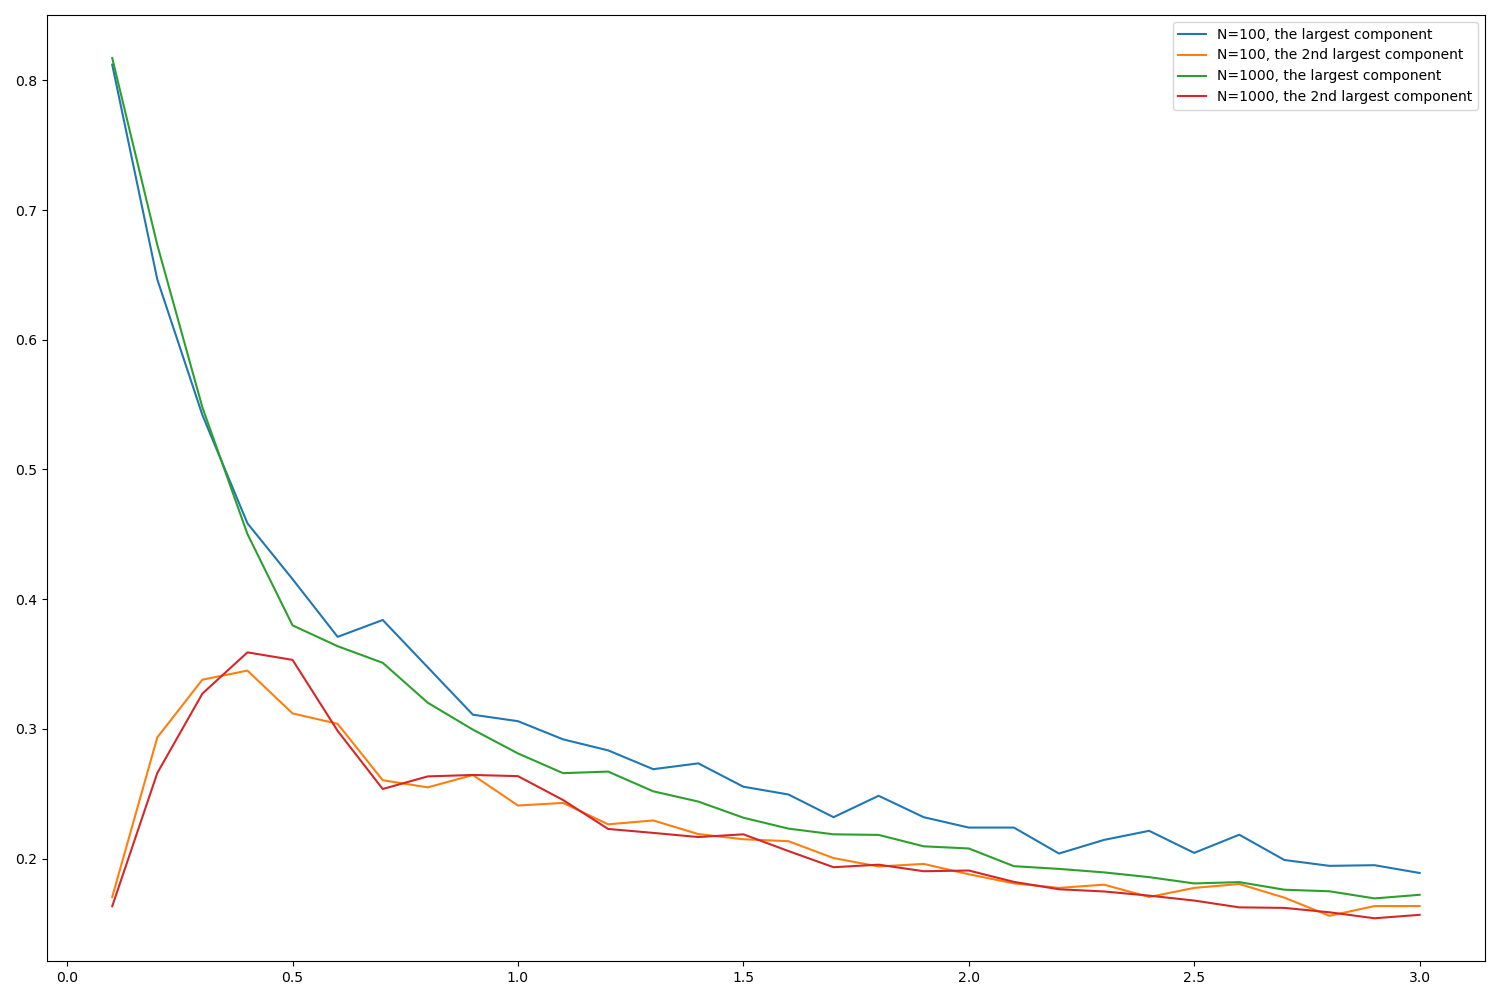
\includegraphics[width=18cm]{./Programming/Q3-3-A.png}
        \caption{The Largest Two Components}
    \end{figure}

    \item[(b)] For $N = 1000$, plot the average local clustering coefficient $\langle C_i \rangle$ against $z$ using all $20$ realizations and $i = 1, \cdots, N$ for averaging, and including error bars indicating the standard deviation for all $20N$ data points.
    
    \textit{ Sol. }
    \lstinputlisting[language=Python]{./Programming/Q3-3-B.py}
    \begin{figure}[htbp]
        \centering
        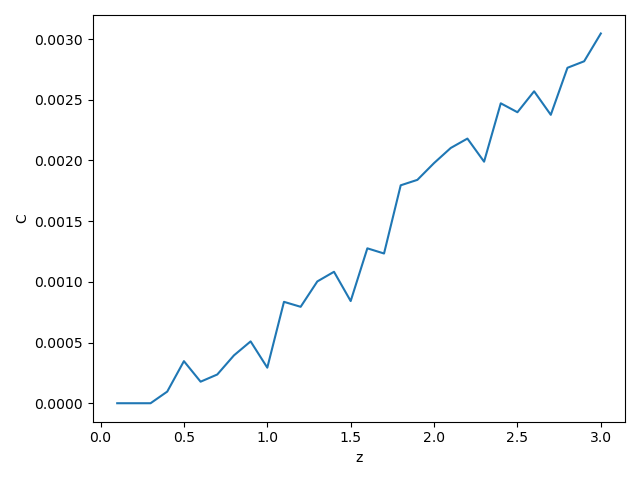
\includegraphics[width=12cm]{./Programming/Q3-3-B.png}
        \caption{The Average of Clustering Coefficients}
    \end{figure}

    \item[(c)] For $N = 1000$ and your favourite value of $z \in [0.5, 2]$, plot the degree distribution $p(k)$ against $k = 0, 1, \cdots$ using $20$ realizations, and compare it to the mass function of the $\text{Poi}(z)$ Poisson distribution in a single plot. 
    
    \textit{ Sol. }
    \lstinputlisting[language=Python]{./Programming/Q3-3-C.py}
    \begin{figure}[htbp]
        \centering
        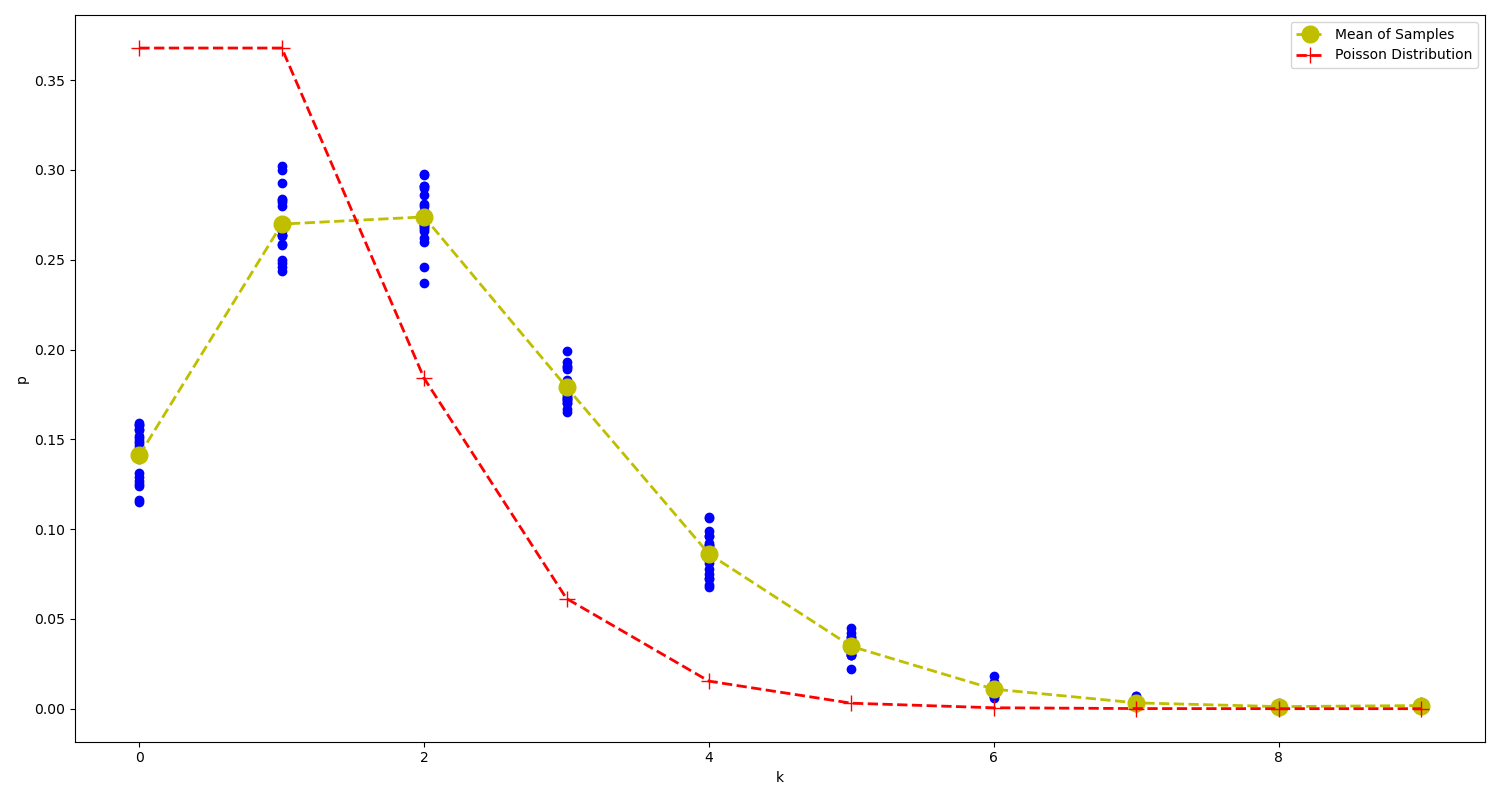
\includegraphics[width=15cm]{./Programming/Q3-3-C.png}
        \caption{Digree Distribution}
    \end{figure}

    \item[(d)] Consider $z = 0.5, 1.5, 5$ and $10$. Plot the spectrum of the adjacency matrix $A$ using all $20$ realizations with a kernel density estimate, and compare it to the Wigner semi-circle law. 
    
    \textit{ Sol. }
    \lstinputlisting[language=Python]{./Programming/Q3-3-D.py}
    \begin{figure}[htbp]
        \centering
        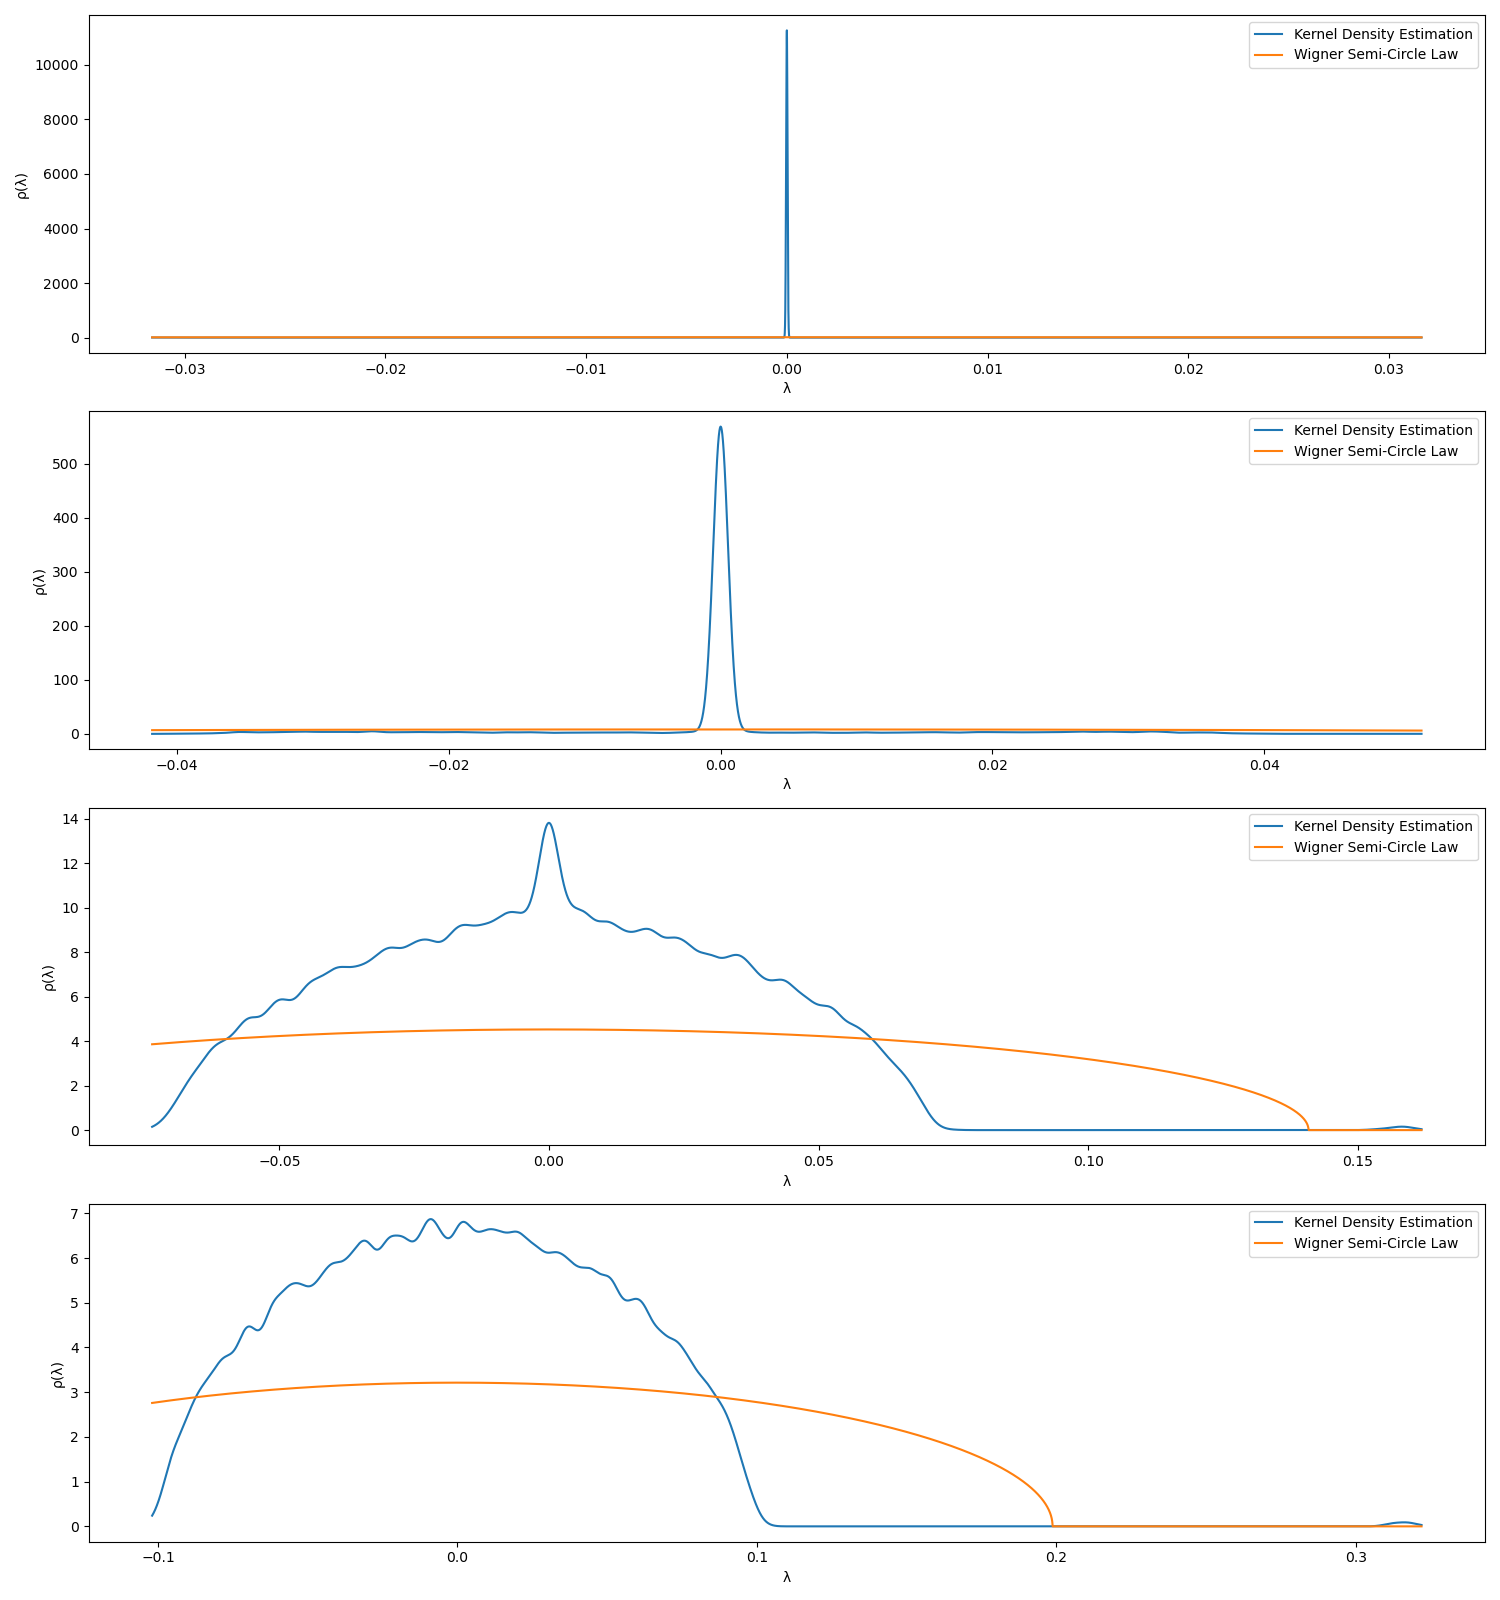
\includegraphics[width=16cm]{./Programming/Q3-3-D.png}
        \caption{Spectrum of the Adjacency Matrix}
    \end{figure}
\end{enumerate}
